\documentclass[14pt, a4paper]{article}
\usepackage[T2A]{fontenc}
\usepackage[utf8]{inputenc}
\usepackage[russian]{babel}
\usepackage[left=3cm, right=1.5cm, top=2cm, bottom=2cm]{geometry}
\usepackage{indentfirst}
\usepackage{microtype}
\usepackage{array}
\usepackage{xcolor}
% \usepackage{times}
\usepackage{tempora}
\usepackage{ulem}
\usepackage{setspace}
\usepackage{amsmath}
\usepackage{booktabs}
\usepackage{graphicx}
\usepackage{float}
\usepackage{listings}
\graphicspath{{reports/figures/}{figures/}}
\lstset{basicstyle=\ttfamily\small, breaklines=true, columns=fullflexible, frame=single, keepspaces=true}
\pagestyle{empty}

\makeatletter
\renewcommand\section{\@startsection {section}{1}{\parindent}%
  {-3.5ex \@plus -1ex \@minus -.2ex}%
  {0.5ex}%
  {\normalfont\Large\bfseries}}
\renewcommand\tableofcontents{%
  \begin{center}\Large\bfseries\contentsname\end{center}%
  \@starttoc{toc}%
}
\renewcommand*\l@section{\@dottedtocline{1}{0em}{1.5em}}
\makeatother

\begin{document}
\onehalfspacing

\begin{center}
    \textbf{ФЕДЕРАЛЬНОЕ ГОСУДАРСТВЕННОЕ АВТОНОМНОЕ ОБРАЗОВАТЕЛЬНОЕ} \\
    \textbf{УЧРЕЖДЕНИЕ ВЫСШЕГО ОБРАЗОВАНИЯ} \\
    \textbf{«МОСКОВСКИЙ АВИАЦИОННЫЙ ИНСТИТУТ} \\
    \textbf{(НАЦИОНАЛЬНЫЙ ИССЛЕДОВАТЕЛЬСКИЙ УНИВЕРСИТЕТ)»}
\end{center}

\begin{center}
    \bfseries Институт №8 «Компьютерные науки и \\
    \bfseries прикладная математика» \\
    \bfseries Кафедра 806 «Вычислительная математика \\
    \bfseries и программирование»
\end{center}

\vspace{3cm}

\begin{center}
    \Large\bfseries Отчет \\
    \vspace{0.5cm}
    \mdseries по лабораторной работе №1.2
\end{center}

\vfill

\noindent
\hfill
\begin{tabular}{ll}
Группа:       & М8О-307Б-21 \\
Студент:      & М. С. Ивченко \\
Преподаватель:& доц. В. В. Киндинова \\
Оценка:       & \underline{\makebox[3cm][c]{}} \\ [0.2cm]
Дата:         & \underline{\makebox[3cm][c]{}}
\end{tabular}

\vfill

\begin{center}
    Москва \\
    2026
\end{center}

\newpage

\setcounter{tocdepth}{2}
\tableofcontents
\newpage

\section*{Тема}
\addcontentsline{toc}{section}{Тема}
Цель данной лабораторной работы -- изучить эффективное решение систем линейных алгебраических уравнений специального вида. Основное внимание уделяется трехдиагональным матрицам, которые часто появляются после разностной аппроксимации дифференциальных задач и позволяют применять компактный метод прогонки.

\section*{Задание}
\addcontentsline{toc}{section}{Задание}
Реализовать метод прогонки в виде программы, задавая в качестве входных данных ненулевые элементы матрицы системы и вектор правых частей. Используя разработанное программное обеспечение, решить СЛАУ с трехдиагональной матрицей.

\section*{Теория}
\addcontentsline{toc}{section}{Теория}
Метод прогонки, или алгоритм Томаса, является специализированным вариантом метода Гаусса для трехдиагональных систем. Такая система имеет вид
\[
    a_i x_{i-1}+b_i x_i+c_i x_{i+1}=d_i.
\]
Все элементы матрицы, кроме главной диагонали и двух соседних диагоналей, равны нулю. Если применять обычный метод Гаусса, большая часть операций будет выполняться с нулями. Метод прогонки использует структуру матрицы и требует только $O(n)$ операций и $O(n)$ памяти.

Алгоритм состоит из прямого и обратного хода. На прямом ходе неизвестная $x_i$ выражается через следующую неизвестную:
\[
    x_i=\alpha_{i+1}x_{i+1}+\beta_{i+1},
\]
где коэффициенты $\alpha_i$ и $\beta_i$ вычисляются последовательно слева направо. Для первой строки
\[
    \alpha_1=-\frac{c_0}{b_0}, \qquad \beta_1=\frac{d_0}{b_0}.
\]
Для внутренних строк после подстановки выражения для $x_{i-1}$ получается
\[
    m_i=b_i+a_i\alpha_i,\qquad
    \alpha_{i+1}=-\frac{c_i}{m_i},\qquad
    \beta_{i+1}=\frac{d_i-a_i\beta_i}{m_i}.
\]
В последней строке находится $x_n$, после чего обратным ходом вычисляются $x_{n-1},\ldots,x_0$ по уже найденной рекуррентной формуле.

Важное условие применимости метода -- отсутствие нулевых знаменателей $m_i$. На практике устойчивость обычно обеспечивается диагональным преобладанием
\[
    |b_i|\ge |a_i|+|c_i|,
\]
причем хотя бы для одной строки неравенство должно быть строгим. Тогда малые ошибки округления не усиливаются резко при прямом и обратном ходе.

\begin{lstlisting}[language=Python]
alpha[1] = -A[0][2] / A[0][1]
beta[1] = b[0] / A[0][1]
for i in range(2, n):
    denom = A[i - 1][0] * alpha[i - 1] + A[i - 1][1]
    alpha[i] = -A[i - 1][2] / denom
    beta[i] = (b[i - 1] - A[i - 1][0] * beta[i - 1]) / denom
for i in reversed(range(n - 1)):
    x[i] = alpha[i + 1] * x[i + 1] + beta[i + 1]
\end{lstlisting}

\section*{Ход лабораторной работы}
\addcontentsline{toc}{section}{Ход лабораторной работы}
Система варианта задавалась тройками $(a_i,b_i,c_i)$:
\[
\begin{array}{c|rrr|r}
i&a_i&b_i&c_i&d_i\\\hline
1&0&-10&-9&7\\
2&-5&-21&-8&29\\
3&7&12&2&31\\
4&0&8&2&56\\
5&2&10&0&-24
\end{array}
\]
После прямого и обратного ходов получено
\[
    x=(2,\;-3,\;3,\;8,\;-4)^T.
\]
Подстановка в исходную систему дает точное совпадение правых частей: например, $-10\cdot2-9\cdot(-3)=7$, $8\cdot8+2\cdot(-4)=56$.

\begin{figure}[H]
    \centering
    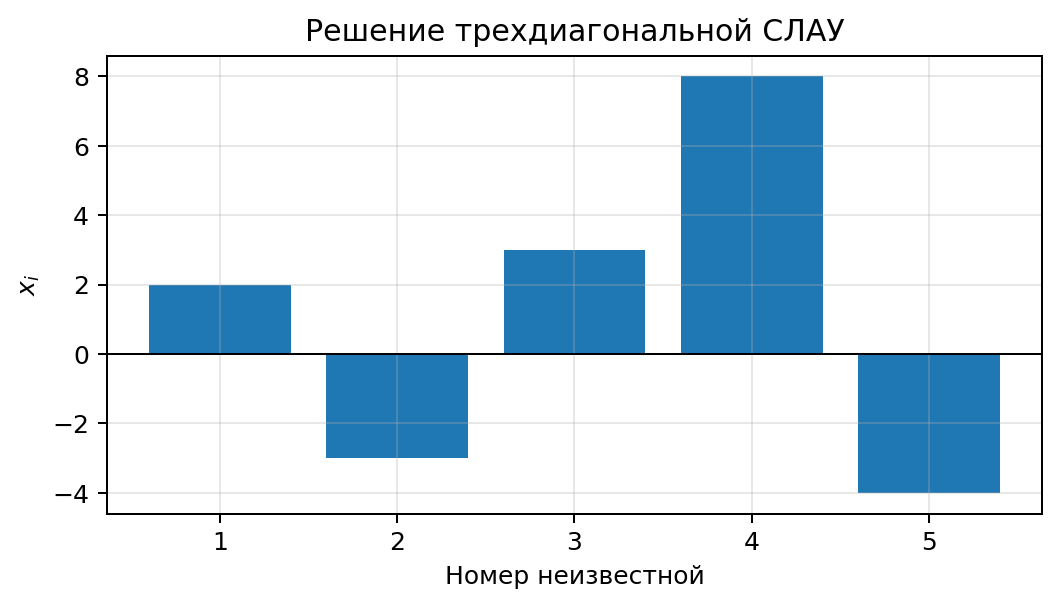
\includegraphics[width=0.86\textwidth]{lab1_2_solution.png}
    \caption{Компоненты решения трехдиагональной системы.}
\end{figure}

\section*{Выводы}
\addcontentsline{toc}{section}{Выводы}
Метод прогонки использует только три диагонали матрицы и решает систему за линейное число операций. Для заданной системы коэффициенты прогонки не обращались в ноль, а найденное решение точно удовлетворяет всем уравнениям.

\end{document}
